\chapter{Étude sur la législation}
\label{ch:etudelegislation}

Ce travail de Bachelor sera effectué en tant que « proof of concept » et ne sera pas utilisé dans le domaine publique,
mais uniquement dans un environnement contrôlé. C’est pourquoi, il ne sera pas affecté par les différentes
contraintes juridiques exprimées dans cette étude.

Toutefois, à titre informatif et pour démontrer la potentielle nocivité d’un tel système, il a été décidé d’effectuer
une étude sur la légalité et la morale de l’utilisation d’outils de traçage.

Il est à noter que le cadre de cette étude ne comprend que la législation suisse. Les libertés individuelles et le lois sur la protection des données divergent beaucoup
d'un pays à l'autre, c'est pourquoi mes conclusions ne sauraient être valides ailleurs. 

\section{Cas d’utilisation}
Pour circonscrire ce travail dans un cadre juridique, il faut se projeter et prédire les use cases princpaux qu’une
solution telle que WiFace pourrait remplir.

Pour rappel, la solution théorique de Wiface permet d’associer une identité (Nom, prénom, adresse, informations
personnelles), un lieu, et un device.

\subsection{Shopping : Publicité ciblée}

Il serait possible, à l’intérieur d’un grand centre commerciel, de placer plusieurs unités de tracking. Ainsi, le nom et
l’adresse d’un client s’attardant régulièrement devant une enseigne permettrait de la publicité extrêmement ciblée.

Les probe requests donnant également des informations complémentaires directes (constructeur) ou indirectes
(modèle du téléphone), il serait possible pour les vendeurs de matériel informatique de cibler de potentiels nouveaux
acheteurs qui auraient un ancien appareil à remplacer dans un futur proche.

\subsection{Analyse de fréquentation d’un espace publique et prédiction de déplacement}

Lors d’un travail de groupe au MIT, des étudiants ont récoltés plusieurs milions de probe requests et on fait une
analyse de fréquentation de divers lieux clés du campus. Leur projet « Arealytics » les a même conduits à prédire
les prochains déplacements d’un individu en fonction de son trajet courant.
\begin{figure}[H]
	\centering
	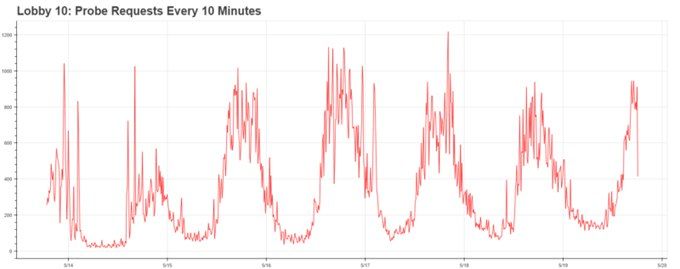
\includegraphics[width=16cm]{images/etude-legi-1.jpg}
	\caption{Arealytics}
	\label{fig:arealytics}
\end{figure}
\begin{figure}[H]
	\centering
	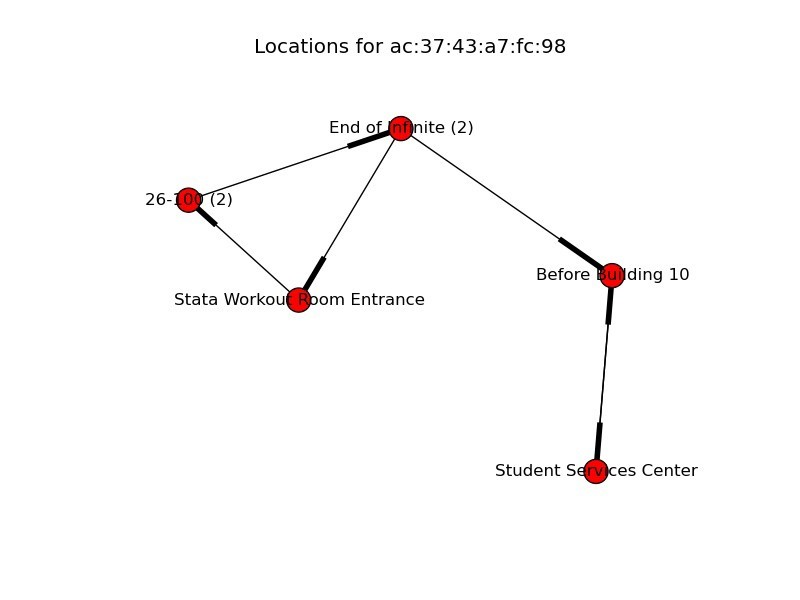
\includegraphics[width=12cm]{images/etude-legi-2.jpg}
	\caption{Arealytics}
	\label{fig:prediction de chemins à l'aide de probe}
\end{figure}

Dans cet exemple, nous voyons que l’utilisation de simple probe request même sans prise d’image donne déjà
énormément d’information brute.

\subsection{Forensique}
La capacité de pouvoir situer un individu, ou un groupe dans un espace géographique donné pourrait être utilisé
comme preuve lors de procès. Par exemple, la présence d’une adresse MAC lors d’un crime, permet, dans une certaine mesure, 
de s’assurer de la présence de l’appareil associé. Couplé à une caméra, cette technique pourrait
singulièrement améliorer les systèmes de surveillance actuels et proposer de nouveaux outils aux enquêteurs.

\section{Définitions}
Selon la Loi fédérale sur la protection des données (LPD) Section 1, Art 3
On entend par:

\begin{enumerate}[label=\alph*]
\item données personnelles (données), toutes les informations qui se rapportent à une personne identifiée ou
identifiable;
\item personne concernée, la personne physique ou morale au sujet de laquelle des données sont traitées;
\item données sensibles, les données personnelles sur:
\begin{enumerate}[label=\alph*]
\item les opinions ou activités religieuses, philosophiques, politiques ou syndicales,
\item la santé, la sphère intime ou l’appartenance à une race,
\item des mesures d’aide sociale,
\item des poursuites ou sanctions pénales et administratives;
\end{enumerate}
\item profil de la personnalité, un assemblage de données qui permet d’apprécier les caractéristiques essentielles
\item la personnalité d’une personne physique;
\item traitement, toute opération relative à des données personnelles – quels que soient les moyens et procédés
utilisés – notamment la collecte, la conservation, l’exploitation, la modification, la communication,
l’archivage ou la destruction de données;
\item communication, le fait de rendre des données personnelles accessibles, par exemple en autorisant leur
consultation, en les transmettant ou en les diffusant;
\end{enumerate}

Ces quelques définitions vont permettre d’aborder les différentes problématiques dressée par ce travail.

\section{Articles affectant le projet}

Dans cette section, il sera fait mention de plusieurs articles de la LPD permettant de justifier – ou non – la potentielle
mise en place du produit en conditions réelles de par sa licéité.

\subsection{Section 1, Art 3, alinéa 2}
« Leur traitement (des données personnelles) doit être effectué conformément aux principes de la bonne foi et de
la proportionnalité. »

Certains des cas d’utilisations mentionnés ne permettent pas de mettre en œuvre le principe de proportionnalité.
Par exemple, utiliser des mécanismes poussés pour découvrir le moyen de contacter un potentiel client sans
intervention de sa part.

\subsection{Section 1, Art 5, alinéa 1}
«Celui qui traite des données personnelles doit s’assurer qu’elles sont correctes. Il prend toute mesure appropriée
permettant d’effacer ou de rectifier les données inexactes ou incomplètes au regard des finalités pour lesquelles
elles sont collectées ou traitées. »

Au vu des algorithmes qui seraient mis en place, il sera difficile voir impossible de garantir l’exactitude des données
personnelles. Par exemple, l’assignation d’une identité à une adresse MAC à l’aide d’image est un processus
hasardeux qui a de grande chance d’aboutir à une mauvaise labellisation des données personnelles

\subsection{Section 3, Art 12, alinéa 2}
«Personne n’est en droit notamment de:
\begin{enumerate}[label=\alph*]
\item traiter des données personnelles en violation des principes définis aux art. 4, 5, al. 1, et 7, al. 1;
\item traiter des données contre la volonté expresse de la personne concernée sans motifs justificatifs;
\item communiquer à des tiers des données sensibles ou des profils de la personnalité sans motifs justificatifs»
Afin de retrouver l’identité d’une personne, la solution WiFace devra communiquer des informations personnelles
à des tiers (e.g recherche inversée d’image).
\end{enumerate}

\section{Conclusion}
Il est apparent que la plupart des cas d’utilisation ne respectent pas la LPD. Par conséquent, l’implémentation
concrète d’une solution comme WiFace semble compromise sur le marché Suisse.


